[10]

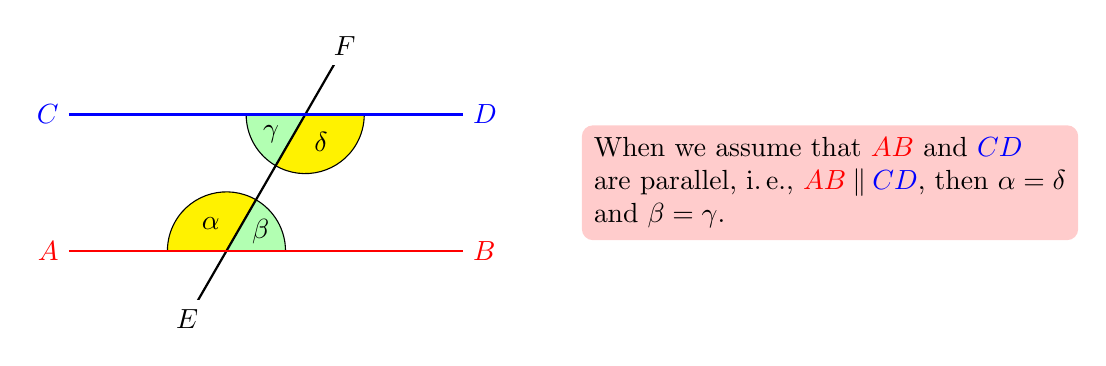
\begin{tikzpicture}
    \draw[fill=yellow] (0,0) -- (60:.75cm) arc (60:180:.75cm);
    \draw(120:0.4cm) node {$\alpha$};

    \draw[fill=green!30] (0,0) -- (right:.75cm) arc (0:60:.75cm);
    \draw(30:0.5cm) node {$\beta$};

    \begin{scope}[shift={(60:2cm)}]
        \draw[fill=green!30] (0,0) -- (180:.75cm) arc (180:240:.75cm);
        \draw (30:-0.5cm) node {$\gamma$};

        \draw[fill=yellow] (0,0) -- (240:.75cm) arc (240:360:.75cm);
        \draw (-60:0.4cm) node {$\delta$};
    \end{scope}

    \begin{scope}[thick]
        \draw (60:-1cm) node[fill=white] {$E$} -- (60:3cm) node[fill=white] {$F$};
        \draw[red]                   (-2,0) node[left] {$A$} -- (3,0)
        node[right]{$B$};
        \draw[blue,shift={(60:2cm)}] (-3,0) node[left] {$C$} -- (2,0)
        node[right]{$D$};

        \draw[shift={(60:1cm)},xshift=4cm]
        node [right,text width=6cm,rounded corners,fill=red!20,inner sep=1ex]
        {
            When we assume that $\color{red}AB$ and $\color{blue}CD$ are
            parallel, i.\,e., ${\color{red}AB} \mathbin{\|} \color{blue}CD$,
            then $\alpha = \delta$ and $\beta = \gamma$.
        };
    \end{scope}
\end{tikzpicture}